%\subsubsection{Problems solved by transformers}
The point of transformers was to overcome the problems faced by the previous state-of-the-art architectures while still including prominent aspects of the RNN and Convolutional Neural Network (CNN) models.

The RNN model has two notable weaknesses. First is its inability to learn long-term patterns, due to the exploding and vanishing gradient problems that occur during backpropagation.
Secondly, its recurrent connection is also a weakness. This is because it is not possible to compute the cell at time step $i$ until the cell at time step $i-1$ has been computed as information is propagated along a sequence.

In contrast, one of the benefits of CNNs is that they can be computed concurrently. However, unlike RNNs, they are unable to learn even short-term patterns. The size of the patterns they can learn is limited by their architecture.

Transformers attempt to feature the best of both techniques.
Transformers can model dependencies over the whole range of the input sequence as easily they can model neighboring sequences. And there are no recurrent connections, allowing efficient computation using parallelization. This is facilitated through the use of the self-attention mechanism.\cite{TransformersScratchPeterbloem}

\begin{figure}[h]
  \centering
  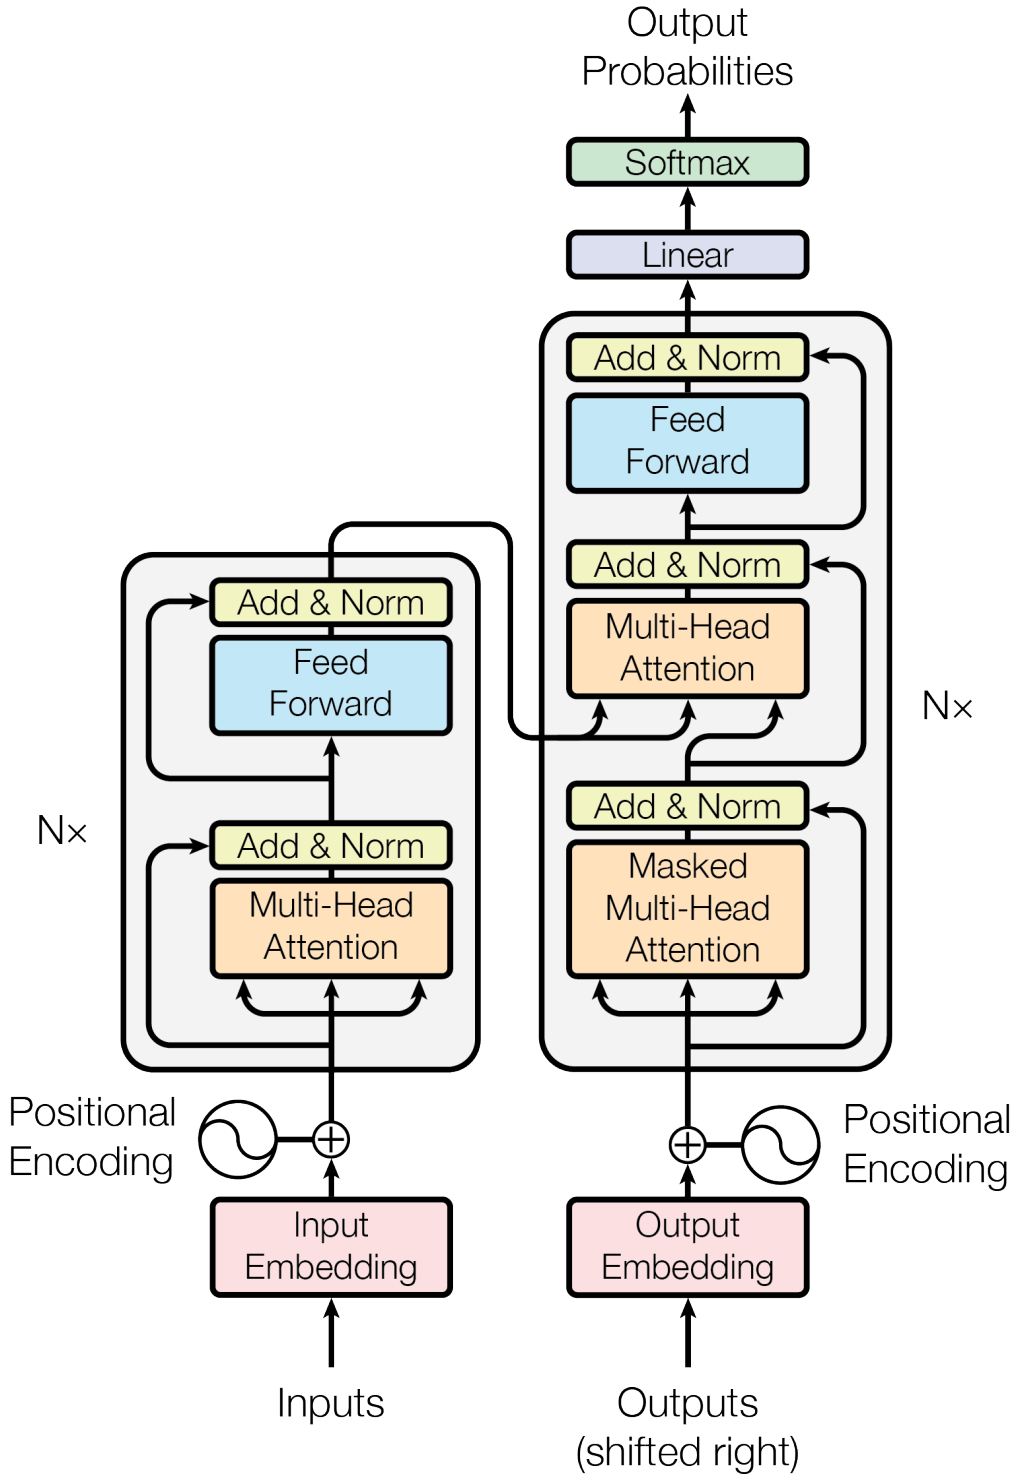
\includegraphics[width=0.5\textwidth]{Transformer model diagram}
  \caption{Diagram depicting the architecture of the transformer model from \citet{AttentionIsAllYouNeed}.}
  \label{fig:original transformer}
\end{figure}
 
\subsection{Self-attention Mechanism}


With self-attention, the model can learn to associate different input.
To achieve this, three input vectors are needed - queries and keys of dimension $d_k$, and values of dimension $d_v$.
The attention function maps the query and the set of key-value pairs to some output, where the output is a weighted sum of the values.
The weight of each value is calculated using a compatibility function.
This weight denotes how compatible the query is with the given key.



The output matrix of weights is computed using the function
$$
Attention(Q, K, V) = softmax(\frac{QK^T}{\sqrt{d_k}})V
$$

Additive attention and dot product attention are among some of the most common attention functions used.
For the purposes of this project, we decided to use the scaled dot product attention technique with the scaling factor $\frac{1}{\sqrt{d_k}}$.
We use this technique as it is faster and more space-efficient as argued in \citet{AttentionIsAllYouNeed}.

Because the dot product can result in values between negative and positive infinity, the \textit{softmax} activation function is used to map values to the interval $[0,1]$, and to ensure that they sum to $1$ over the entire sequence. \cite{AttentionIsAllYouNeed}

\subsection{Multi-Head Attention} \label{sec:multi-head attention}
To improve the self-attention mechanism, the authors of the original transformer model implemented multi-head attention.
This is a module that runs through the previously described attention mechanism multiple times and in parallel.
It then concatenates the attention weights of all the independent self-attention layers. 

\begin{align*}
MultiHead(Q, K, V) = Concat(h_1, \ldots, h_i)W^O \\
\text{where }h_i = Attention(QW^Q_i, KW^K_i, VW^V_i) 
\end{align*}

In the model we use, the weights are then passed through a dense layer in which a non-linear transformation is applied using the \textit{ReLU} activation function rather than a linear transformation as described in \citet{AttentionIsAllYouNeed}. 
Once this computation is completed, the result is the final multi-head attention weight matrix. \cite{AttentionIsAllYouNeed}

\subsection{Time embedding}
The transformer model is indifferent to temporal information.
Therefore, in order to embed our temporal data, we convert the input data to a vector representation.
Furthermore, vector representations are used for many different tasks, making a vector representation for time easily usable with a variety of different architectures.

To this end, we use the approach described in \citet{time2vec}. 
This paper conveys two main ideas.
Firstly, the time representation should contain both periodic and non-periodic information.
Secondly, the time representation should not be affected by different time increments and long time horizons.  

For a given scalar notion of time $\tau$, TimeToVector of $\tau$ is a vector of size $k + 1$ with the following definition: \\

\begin{math}
  TimeToVector(\tau)[i]=\left\{
    \begin{array}{ll}
      \omega_i \tau + \varphi_i, & \mbox{if $x<0$}.\\
      \mathcal{F}(\omega_i \tau + \varphi_i), & \mbox{if $1 \le i \le k$}.
    \end{array}
  \right.\\
\end{math}

where $TimeToVector(\tau)[i]$ is the \textit{i}th element of $TimeToVector(\tau)$, $\mathcal{F}$ is a periodic activation function (the sine function, in our case), and $\omega_i$ and $\varphi_i$ are learnable parameters. 

For $\mathcal{F} = sin, 1 \leq i \leq k$, $\omega_i$ is the frequency and $\varphi_i$ is the phase-shift.
Since the sine function is periodic, $\tau$ has the same value as $\tau + \frac{2\pi}{\omega_i}$, which helps capture periodic behavior without any feature engineering.
An example of this is the sine function $sin(\omega\tau + \varphi)$ with $\omega = \frac{2\pi}{7}$ can be used to model weekly patterns, assuming $\tau$ denotes days.
It is worth noting that the authors of the paper chose the sine function due to experiments showing that models using it outperform models that use non-periodic activation functions instead.\cite{time2vec}


%- forklar hvad dropout layer gør
%- forklar hvad residual connection gør
%- forklar hvad normalization gør
\subsection{The transformer encoder layer}\label{sec:transformer encoder}
The previously described elements are now aggregated into a transformer encoder layer.
To improve the performance of the transformer, multiple of these layers can be stacked, and each of these encoder layers contain a self-attention sublayer as well as a feedforward sublayer. 

Once the multi-head attention weights have been computed, these weights are then fed into a dropout layer that has a residual connection consisting of the initial query.
Given some rate value, this layer randomly sets the input units to 0 using that rate as the frequency.
In other words, some values from the input are dropped, which helps prevent overfitting during training.

Following the dropout layer, the weights are normalized in a normalization layer. 
This gives us the final attention weights which are then passed to the feedforward layer.

The feedfoward layer is the dense layer, as described in section \ref{sec:multi-head attention}.
It should be noted that the two dense layers per encoder layer consist of 1-dimensional convoluted neural networks with a kernel size and stride of 1.
The output of these two layers are then fed into another dropout layer, which also has a residual connection consisting of the initial query. 

Finally, the values are normalized, which gives us the final transformer encoder output values.
The resulting architecture can be seen in figure \ref{fig:encoder transformer}.
As this figure demonstrates, the architecture is different from the original transformer architecture shown in \ref{fig:original transformer}.
Our transformer architecture is based on the architecture by \citet{schmitz_stock_2020}, which includes many of the original architectural elements from \textit{Attention Is All You Need} \cite{AttentionIsAllYouNeed}.
Because we are not working with natural language processing, there is no need for a decoder layer, since we do not to output any decoded data. 

\begin{figure}[h]
\centering
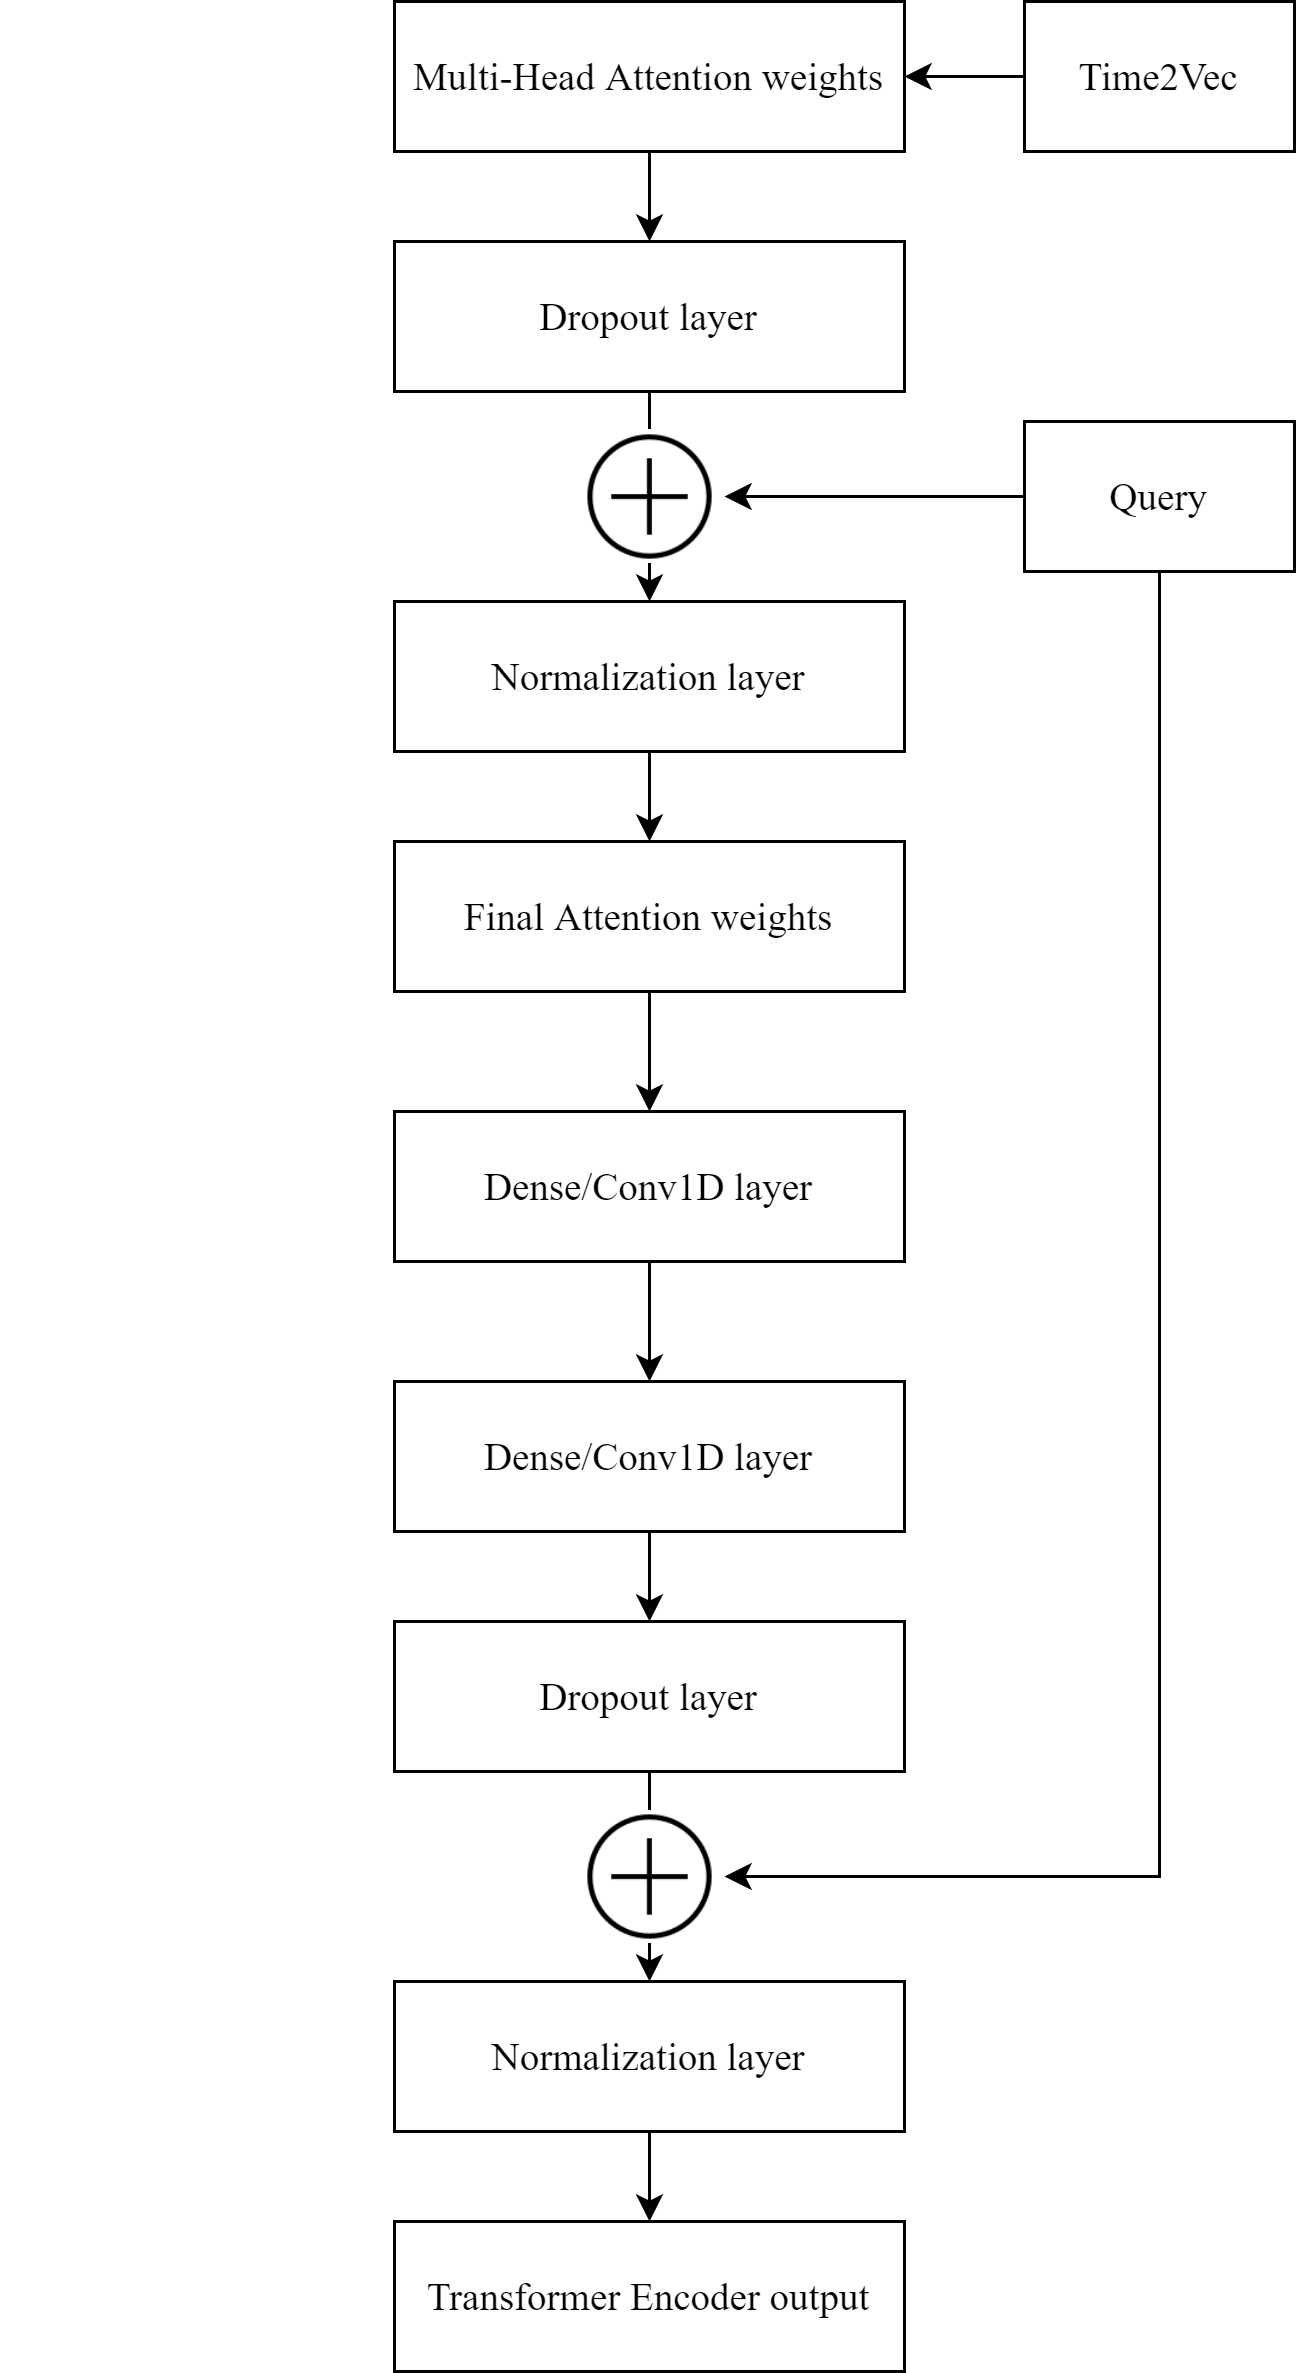
\includegraphics[width=0.45\textwidth]{Encoder transformer}
\caption{The transformer encoder layer.}
\label{fig:encoder transformer}
\end{figure}